\documentclass{beamer}
\usecolortheme{whale}
\usepackage[utf8]{inputenc}
\usepackage{dirtytalk,amsmath,tikz,mathtools,amsmath}
\usepackage{resizegather}
\usetikzlibrary{automata, positioning}
\graphicspath{ {./images/} }
\tikzset{->, initial text=$$}
%Information to be included in the title page:
\title{Logic and Hybrid Systems}
\author{Manasvi Saxena}
\institute{Formal Systems Lab, UIUC}
\date{}

\setbeameroption{hide notes} % Only slides
%\setbeameroption{show only notes} % Only notes
%\setbeameroption{show notes on second screen=right} % Both
\setbeamertemplate{note page}{\pagecolor{yellow!5}\insertnote}\usepackage{palatino}
\setbeamerfont{caption}{size=\scriptsize}

\newcommand{\dL}{\text{\upshape\textsf{d{\kern-0.05em}L}}}
\newcommand{\Trm}{\text{Trm}}
\newcommand{\HP}{\text{HP}}
\newcommand{\accel}{\textit{accel}}
\newcommand{\brake}{\textit{brake}}

\begin{document}

\frame{\titlepage}

\begin{frame}
\frametitle{Hybrid Systems}

\begin{itemize}
  \item Dynamical Systems exhibiting both discrete (jump) and continuous (flow) behaviors.
  \item Serve as models of physical systems, from thermostats to trains.
  \item Continuous dynamics specified using Differential Equations.
\end{itemize}

\end{frame}

\begin{frame}
  \frametitle{Differential Dynamic Logic (\dL)}
  \begin{itemize}
    \item Main focus - Differential Dynamic Logic for Hybrid Systems (Andre
      Platzer).
      \pause
    \item Practical deductive verification of hybrid systems.
      \pause
    \item Introduces Hybrid Program - program notation for hybrid systems.
      \pause
    \item Dynamic Logic for Hybrid Programs, a generalization of Dynamic Logic.
      \pause
    \item Suited for automation.
  \end{itemize}

\end{frame}

\begin{frame}
\frametitle{Hybrid Automata}
\begin{itemize}
  \item Commonly used to model Hybrid Systems, via Graphs.
  \item Nodes specify continuous dynamics. Edges describe discrete transitions.
  \item Intuitive, but not suitable for deductive verification.
\end{itemize}
    \pause
\begin{figure}\label{fig:train-HA}
  \centering
  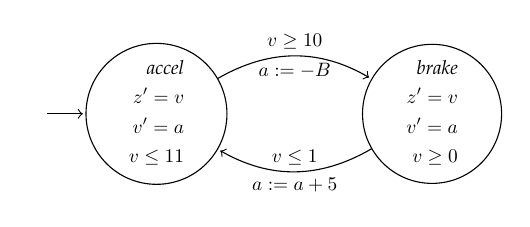
\begin{tikzpicture}[shorten >=1pt,node distance=5cm,on grid,auto]
    
  \node[state,initial, scale=0.70] (accel)   {%
  $\begin{aligned}
      \textit{accel} \\
      z' = v \\
      v' = a \\
      v \leq 11
  \end{aligned}$
  };

  \node[state,scale=0.70] (brake) [right of = accel] {%
  $\begin{aligned}
      \textit{brake} \\
      z' = v \\
      v' = a \\
      v \geq 0
  \end{aligned}$
   };

   \draw (accel) edge[bend left, above] node[midway,below,scale=0.7] {$a := -B$}
   node[midway,above,scale=0.7] {$v \geq 10$} (brake);
   \draw (brake) edge[bend left, below] node[midway,below,scale=0.7] {$a := a+5$}
   node[midway,above,scale=0.7] {$v \leq 1$} (accel);

  \end{tikzpicture}
  \caption{Hybrid Automata (simplified) of a Train Control System}
\end{figure}
\end{frame}

\begin{frame}{Differential Dynamic Logic}{Motivations}
  \begin{itemize}
    \item \textbf{First Order Logic} - No builtin means for referring to state
      transitions.
    \item \textbf{Temporal Logics} - Modal operators allow referring to state transitions.
      But valid formulas only express generic facts.
      \pause
    \item \textbf{Dynamic Logic (DL)} - Combines operational system models with
      operators for reasoning.
      \begin{itemize}
        \item Provides parameterized modal operators, $[\alpha]$,
          $\langle\alpha\rangle$
          that refer to states reachable by system $\alpha$.
        \item $[\alpha]\phi$ expresses all states reachable by $\alpha$ satisfy
          $\phi$, allowing reasoning about discrete systems.
        \item Say $(b > 0) \to [a := -b] (a < 0) $ expresses a
          discrete transition. We can prove $(b > 0) \vdash (a < 0) [ b / a ]$
          using DL's calculus.
        \item No built in notion for describing or reasoning about continuous dynamics.
      \end{itemize}
  \end{itemize}
\end{frame}

\begin{frame}{Differential Dynamic Logic}{Motivations}
  \begin{itemize}
    \item Generalize DL so operational models $\alpha$ can be
      used in modal formulas like $[\alpha]\phi$. $\dL$ refers to
      generalized models as \say{Hybrid Programs}.
    \item A compositional calculus for verification. Decompose
      $[\alpha]\phi$ into an equivalent formula $[\alpha_1]\phi_1 \wedge
      [\alpha_2]\phi_2$.
    \item Prove subsystems and subproperties $[\alpha_i]\phi_i$ independently
      and combine results conjuntively.
    \item Complete relative to handling of differential equations.
  \end{itemize}
\end{frame}

\begin{frame}{Differential Dynamic Logic}{Syntax and Semantics}
    $\dL$ formulas built over
    \begin{itemize}
      \item $V$, set of real-valued logical variables and
     signature $\Sigma$ containing functions, predicate symbols over reals, like
     $0, 1, +, \geq$.
   \item Signature $\Sigma$ containing functions and predicates, like $0, 1
     \geq$.  $\Sigma$ also contains \textit{System State Variables}. Unlike rigid
   symbols, like $1, 2$, their interpretation can change from state to state.
 \item Set $\text{Trm}(\Sigma,V)$ of \textit{terms} defined as classical FOL polynomial (or
   rational) expressions over $V$ with additional skolem terms $s(X_1, \dots,
   X_n)$, where $X_1, \dots, X_n \in V$.
 \end{itemize}
\end{frame}

\begin{frame}{Differential Dynamic Logic}{Syntax and Semantics}
  \begin{block}{Hybrid Programs}
  Consider $x_i \in \Sigma$, $\theta_i, \vartheta_i \in \Trm(\Sigma, V)$ for
  $1 \leq i \leq n$, $\chi$ a $(\Sigma,V)$ FOL-formula, $\alpha, \beta \in
  \HP(\Sigma,V)$
    Set $\HP(\Sigma,V)$, is defined inductively as -
    \begin{itemize}
      \item  $(x_1 := \theta_1, \ldots , x_n = \theta_n) \in \HP(\Sigma,V)$
      \item $ (x'_1 = \vartheta_i, \ldots , x'_n = \theta_n)\, \& \, \chi \in
        \HP(\Sigma,V)$. $x'_i = \vartheta_i$ is a differential equation where
        $x'_i$ is the first order time derivative of $x_i$.
      \item $(?\chi) \in \HP(\Sigma,V)$.
      \item $\alpha \cup \beta \in \HP(\Sigma, V)$.
      \item $\alpha;\beta \in \HP(\Sigma, V)$.
      \item $\alpha^* \in \HP(\Sigma, V)$.
    \end{itemize}
  \end{block}
\end{frame}


\begin{frame}{Differential Dynamic Logic}{Hybrid Program Example}
    \begin{columns}
    \uncover<1,2>{%
    \column{.4\textwidth}
      \begin{figure}
      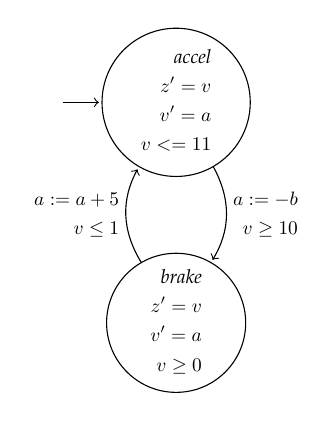
\begin{tikzpicture}[shorten >=1pt,node distance=4cm,on grid,auto]
        
  \node[state,initial, scale=0.70] (accel)   {%
  $\begin{aligned}
      \textit{accel} \\
      z' = v \\
      v' = a \\
      v <= 11
  \end{aligned}$
  };

  \node[state,scale=0.70] (brake) [below of = accel] {%
  $\begin{aligned}
      \textit{brake} \\
      z' = v \\
      v' = a \\
      v \geq 0
  \end{aligned}$
   };

   \draw (accel) edge[bend left, left] node[right,scale=0.7](t1) {%
     $\begin{aligned}
       a := -b \\
       v \geq 10
     \end{aligned}$
   } (brake) ;
   \draw (brake) edge[bend left, right] node[left,scale=0.7](t2) {%
     $\begin{aligned}
       a := a + 5 \\
       v \leq 1
     \end{aligned}$
   }(accel);

      \end{tikzpicture}
      \caption{Hybrid Automata of Simple Train Control System}
      \end{figure}
    }
    \uncover<2>{%
    \column{.6\textwidth}
    \begin{equation*}
    \begin{split}
      & q := \accel; \\
      & ( (?q = \accel; z' = v,v' = a) \\
      &  \cup (?q = \accel \wedge z \geq s; a := - b; q:=\brake; ?v \geq 0) \\
      &  \cup (?q = \brake; z' = v,v' =a \& v \geq 0) \\
      &  \cup (?q = \brake \wedge \leq 1; a := a + 5; q:=\accel) )*
      \end{split}
    \end{equation*}
  }
    \end{columns}
\end{frame}

\end{document}

